\begin{figure*}[t]
    \centering
    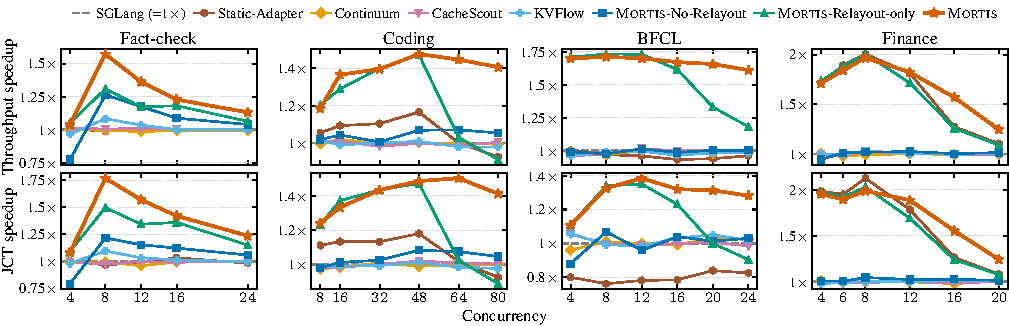
\includegraphics[width=0.95\textwidth]{figures/decomposed_graphs/per-agent/raw_baselines/speedup.pdf}
    \vspace{-8pt}
    \caption{Throughput speedup (top) and average JCT speedup (bottom) over SGLang on each agent workload under varying concurrency.}
    \vspace{-8pt}
    \label{fig:e2e_speedup}
\end{figure*}

\section{Evaluation}
\label{sec:eval}
\subsection{Experimental Setup}
\para{Testbed and model}
We implement \sysname on top of SGLang v0.5.10.post1 and conduct evaluations on one A40 GPU using Qwen3-32B-AWQ. We allocate 15\,GB of GPU memory and 25\,GB of CPU memory to the device and host KV-cache pools. 

\para{Baselines}
We compare \sysname against five baselines, reimplemented on our SGLang fork:
\begin{enumerate*}[label=\textbf{(\roman*)}]
    \item \textbf{SGLang}~\cite{zheng2024sglang}, the vanilla SGLang engine with HiCache and default LRU eviction;
    \item \textbf{CacheScout}~\cite{zhang2026cachescout}, which learns call transitions online to prioritize and prefetch agent prefixes;
    \item \textbf{Continuum}~\cite{li2025continuum}, which pins agent KV-cache across tool gaps using adaptive TTLs;
    \item \textbf{KVFlow}~\cite{pan2025kvflow}, which schedules prefix eviction and prefetching via an Agent Step Graph; and
    \item \textbf{Static-Adapter}, which mirrors DSPy's adapter~\cite{dspy2026chatadapter} by hoisting invariant components to the front under a fixed, program-agnostic layout.
\end{enumerate*}

We also evaluate the following ablation variants of \sysname:
\begin{enumerate*}[label=(\roman*)]
    \item \textbf{\sysname-Relayout-only} enables adaptive prompt re-layout but replaces proactive KV-cache scheduling with LRU eviction;
    \item \textbf{\sysname-No-Relayout} enables proactive KV-cache scheduling but disables adaptive prompt re-layout; and
    \item \textbf{\sysname-No-Prefetch} disables only KV-cache prefetching.
\end{enumerate*}
Additionally, we run baseline serving systems on top of \sysname's re-layout to isolate scheduling policy under the same prompt layout.

\para{Workloads}
We evaluate \sysname on four representative agent workloads, ported to Jac byLLM~\cite{mars2023jaseci}: a HoVer-style~\cite{jiang2020hover} Fact-check agent, a HumanEval~\cite{chen2021evaluating} coding agent, a BFCL~\cite{patil2025bfcl} tool-use agent, and a FinanceBench~\cite{islam2023financebench} financial-analysis agent. We further evaluate a mixed workload comprising all four agent types to assess \sysname's end-to-end performance under concurrent, heterogeneous demand. 


\subsection{End-to-End Performance of \sysname}
We test \sysname under different numbers of concurrent workflows and on a mixed workload. Across these workloads, we compare the average job completion time (JCT) and throughput (prompt tokens served per minute).


\para{Performance on different workload types}
As shown in Figure~\ref{fig:e2e_speedup}, \sysname achieves a 1.08--1.99$\times$ JCT speedup and increases throughput by 1.04--1.97$\times$ compared with SGLang, with geometric-mean gains of 1.45$\times$ in JCT and 1.49$\times$ in throughput. Across these agents, serving systems such as KVFlow show no significant improvement, because they ignore intra-prompt heterogeneity. 

Under low concurrency, adaptive prompt re-layout accounts for nearly all of the improvement, because memory is sufficient. As load increases, however, the KV-cache becomes contested. Without knowing what to keep and what to give up, other serving systems fail to schedule it efficiently. 

For the financial-analysis agent, \sysname's improvement is small, because this agent is a simple pipeline that digests large blobs of documents. Under low pressure, adaptive prompt re-layout accounts for nearly all of the improvement by exposing larger prefix reuse. \sysname's proactive KV-cache scheduling only takes effect under the highest load, because it can proactively evict stale KV-cache entries. 

\para{Performance on mixed workload}
We evaluate \sysname under varying pressure on the mixed workload and report metrics over each system's steady-state window. We vary the number of lanes (concurrent workflows) per agent, keeping it equal across all four agents.

As shown in Figure~\ref{fig:lane_sweep}, \sysname achieves up to 1.86$\times$ throughput speedup and 1.83$\times$ JCT speedup over SGLang at 3 lanes per agent. Under low pressure, adaptive prompt re-layout alone accounts for nearly all of the gain, since device memory is still large enough to retain the reusable KV-cache. As pressure grows, the cache becomes contested and the gain from re-layout alone shrinks, while proactive KV-cache scheduling retains a clear advantage by protecting the reusable heads that LRU would evict. Under the heaviest pressure, configurations converge toward the baseline, as the engine is fully saturated and no free memory is left for cache management to exploit. Across the six lane counts, \sysname achieves geometric-mean speedups of 1.56$\times$ in throughput and 1.53$\times$ in JCT.

In the mixed workload, agents have heterogeneous demands for KV-cache memory, which reduces the chance that they contend for memory at the same time. By exploiting intra-prompt heterogeneity, \sysname can promptly yield stale KV-cache to other requests that need memory, which further amplifies the benefit of \sysname.

\begin{figure}[tb]
    \centering
    \captionsetup[subfigure]{font=footnotesize,skip=1pt,margin=-6pt}
    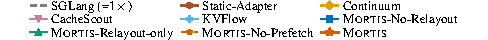
\includegraphics[width=\columnwidth]{figures/decomposed_graphs/mixed/raw_baselines/legend.pdf}\\[1pt]
    \begin{subfigure}[t]{0.333\columnwidth}
        \centering
        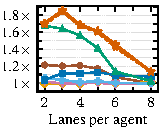
\includegraphics[width=\linewidth]{figures/decomposed_graphs/mixed/raw_baselines/throughput_speedup.pdf}
        \caption{Throughput speedup}
        \label{fig:lane_sweep_tp}
    \end{subfigure}%
    \begin{subfigure}[t]{0.333\columnwidth}
        \centering
        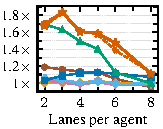
\includegraphics[width=\linewidth]{figures/decomposed_graphs/mixed/raw_baselines/jct_speedup.pdf}
        \caption{JCT speedup}
        \label{fig:lane_sweep_jct}
    \end{subfigure}%
    \begin{subfigure}[t]{0.333\columnwidth}
        \centering
        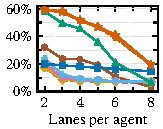
\includegraphics[width=\linewidth]{figures/decomposed_graphs/mixed/raw_baselines/hit_rate.pdf}
        \caption{Cache hit rate}
        \label{fig:lane_sweep_hit}
    \end{subfigure}
    \vspace{-6pt}
    \caption{Throughput and JCT speedup over SGLang and cache hit rate under varying lanes per agent on the mixed workload. JCT speedup is the geometric mean of the four agents' speedups.}
    \label{fig:lane_sweep}
    \vspace{-8pt}
\end{figure}

\para{Task quality} The performance gains of \sysname do not come at the cost of task quality. As shown in Table~\ref{tab:layout_accuracy}, across three different layouts produced by the original byLLM, Static-Adapter, and \sysname, reordering components does not harm task quality.

\begin{table}[tb]
    \centering
    \caption{Task accuracy under three prompt layouts that appear in our evaluation.}
    \label{tab:layout_accuracy}
    \resizebox{\linewidth}{!}{%
        \begin{tabular}{lcccc}
            \toprule
            Prompt layout & Fact-check & Coding & Financial-analysis & BFCL \\
            \midrule
            Original byLLM & 16.3\% & 55.3\% & 34.9\% & 14.1\% \\
            \sysname & 21.9\% & 54.8\% & 37.2\% & 18.7\% \\
            Static-Adapter  & 16.3\% & 52.2\% & 37.8\% & 16.0\% \\
            \bottomrule
        \end{tabular}%
    }
    \vspace{-8pt}
\end{table}

\begin{figure}[tb]
    \centering
    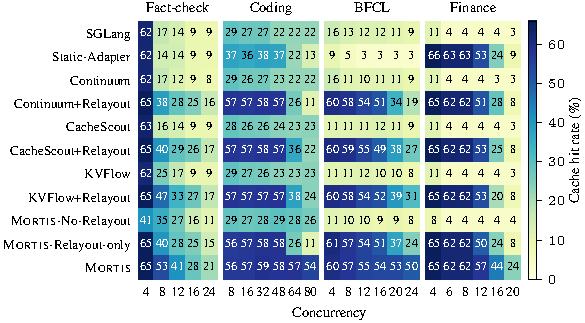
\includegraphics[width=\columnwidth]{decomposed_graphs/per_agent_hit_rate.pdf}
    \caption{Cache hit rate (\%) of prompt tokens under varying concurrency}
    \vspace{-8pt}
    \label{fig:hit_rate}
\end{figure}

\subsection{Cache Efficiency of \sysname}
Figure~\ref{fig:hit_rate} shows the cache hit rate of prompt tokens at the same concurrency levels as Figure~\ref{fig:e2e_speedup}. On Coding and BFCL, adaptive prompt re-layout alone brings the hit rate at low concurrency to that of \sysname: it places the stable and shared bindings at the front, where they form a reusable head that later calls hit. As concurrency grows, the hit rate of \sysname-Relayout-only drops quickly, because LRU eviction does not distinguish reusable heads from volatile tails. With proactive KV-cache scheduling, \sysname keeps a higher hit rate than \sysname-Relayout-only as concurrency grows, and on Coding its hit rate stays nearly flat. On the Fact-check agent, \sysname's hit rate exceeds that of \sysname-Relayout-only from the lowest concurrency. Continuum and CacheScout stay close to SGLang at every concurrency. \sysname-No-Relayout stays below \sysname, since under the original prompt order the reusable head is short. The mixed workload shows a similar pattern (Figure~\ref{fig:lane_sweep}).

\subsection{Ablation Study}
As the geometric-mean speedups of JCT and throughput over SGLang on the four workloads in Table~\ref{tab:complementary} show, \emph{adaptive prompt re-layout} and \emph{proactive KV-cache scheduling} are superadditive: when both are enabled, the speedup is higher than the product of the two individual speedups. The same effect appears on the mixed workload (Figure~\ref{fig:lane_sweep_tp}), where adding proactive KV-cache scheduling on top of adaptive prompt re-layout substantially improves performance.

The gain of \sysname's KV-cache scheduling builds on re-layout, because re-laying out the prompt order exposes a reusable prefix and a suffix that can be abandoned. \sysname's KV-cache scheduling substantially improves performance on top of re-layout, but scheduling alone (\sysname-No-Relayout) barely helps (Table~\ref{tab:complementary}). The same trend appears in Figures~\ref{fig:lane_sweep} and \ref{fig:e2e_speedup}.

Prefetching contributes little on this testbed. As shown in Figure~\ref{fig:lane_sweep_tp}, disabling it (\sysname-No-Prefetch) lowers throughput by at most 2.6\% across the six lane counts. The gain of proactive KV-cache scheduling mainly comes from retention, which keeps the reusable heads resident.

\begin{table}[t]
    \centering
    \caption{Geometric-mean speedup over SGLang across all concurrency levels of the four agent workloads, with \emph{Adaptive Prompt Re-layout} and \emph{Proactive KV-cache Scheduling} on or off.}
    \label{tab:complementary}
    \small
    \setlength{\tabcolsep}{4pt}
    \begin{subtable}[t]{0.49\columnwidth}
        \centering
        \caption{JCT speedup}
        \begin{tabular}{lcc}
        \toprule
         & \multicolumn{2}{c}{Scheduling} \\
        \cmidrule(lr){2-3}
        Re-layout & Off & On \\
        \midrule
        Off & 1.00$\times$ & 1.03$\times$ \\
        On  & 1.30$\times$ & 1.45$\times$ \\
        \bottomrule
        \end{tabular}
    \end{subtable}
    \hfill
    \begin{subtable}[t]{0.49\columnwidth}
        \centering
        \caption{Throughput speedup}
        \begin{tabular}{lcc}
        \toprule
         & \multicolumn{2}{c}{Scheduling} \\
        \cmidrule(lr){2-3}
        Re-layout & Off & On \\
        \midrule
        Off & 1.00$\times$ & 1.02$\times$ \\
        On  & 1.36$\times$ & 1.49$\times$ \\
        \bottomrule
        \end{tabular}
    \end{subtable}
    \vspace{-8pt}
\end{table}

\subsection{Comparison under Identical Layouts}
Serving the baseline systems with re-laid prompts identical to \sysname's, we evaluate their speedup against \sysname-Relayout-only. As shown in Figure~\ref{fig:mixed_baseline_relayout}, these systems show marginal improvement over \sysname-Relayout-only, but are still beaten by \sysname. We further evaluate on the four agent workloads separately. Figure~\ref{fig:speedup_baseline_relayout} shows the same trend as in Figure~\ref{fig:mixed_baseline_relayout}. The largest gains are from CacheScout on Coding and KVFlow on Fact-check, both up to 1.11$\times$ in JCT, but \sysname still outperforms all of them.

This deficiency in baseline serving systems arises because they manage the KV-cache only at the granularity of a prefix and its suffix, which ignores intra-prompt heterogeneity. They cannot identify precisely which KV-cache entries will be reused, leading to inefficient KV-cache scheduling.

\begin{figure}[t]
    \centering
    \captionsetup[subfigure]{font=footnotesize,skip=1pt}
    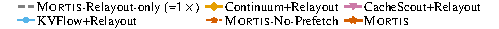
\includegraphics[width=\columnwidth]{figures/decomposed_graphs/per-agent/relayout+baselines/legend_shared.pdf}\\[1pt]
    \begin{subfigure}[t]{\columnwidth}
        \centering
        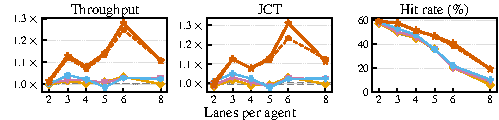
\includegraphics[width=\linewidth]{figures/decomposed_graphs/per-agent/relayout+baselines/mixed.pdf}
        \caption{Throughput, JCT speedup and hit rate on the mixed workload}
        \label{fig:mixed_baseline_relayout}
    \end{subfigure}\\[1pt]
    \begin{subfigure}[t]{\columnwidth}
        \centering
        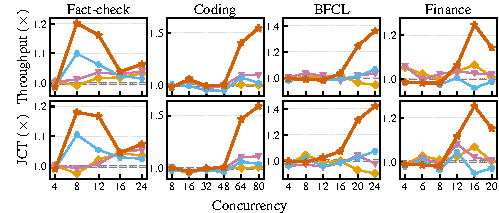
\includegraphics[width=\linewidth]{figures/decomposed_graphs/per-agent/relayout+baselines/speedup.pdf}
        \caption{Throughput and JCT speedup on each agent workload}
        \label{fig:speedup_baseline_relayout}
    \end{subfigure}
    \vspace{-6pt}
    \caption{Baseline systems served with \sysname's re-laid prompts. Speedups are measured against \sysname-Relayout-only.}
    \vspace{-8pt}
\end{figure}


\subsection{Sensitivity Study}


We further run the mixed workload on four A40 GPUs with TP=4 and the same KV-cache pool size. TP=4 increases the prefill speed by 1.74$\times$ (from 1292.4 to 2251.8 tokens/s), which lowers the cost of a cache miss. As shown in Figure~\ref{fig:tp4}, \sysname maintains its advantage even under cheaper cache misses. It achieves geometric-mean speedups of 1.60$\times$ in throughput and 1.58$\times$ in JCT (up to 1.92$\times$ and 1.87$\times$).  

\begin{figure}[t]
    \centering
    
\includegraphics[width=\columnwidth]{figures/TP=4/legend.pdf}\\[1pt]
    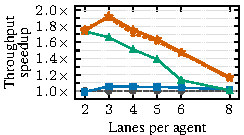
\includegraphics[width=0.5\columnwidth]{figures/TP=4/throughput_speedup.pdf}%
    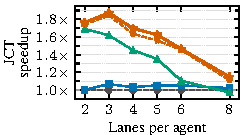
\includegraphics[width=0.5\columnwidth]{figures/TP=4/jct_speedup.pdf}
    \vspace{-6pt}
    \caption{Speedup over SGLang under mixed workload, A40 TP=4}
    \label{fig:tp4}
    \vspace{-8pt}
\end{figure}
% \sysname's performance optimization comes from more efficient KV-cache scheduling. The advantage of \sysname does not disappear or shrink when a cache miss is cheaper. Trends under TP=4 in Figure~\ref{fig:tp4} show the same pattern as in Figure~\ref{fig:lane_sweep}. \sysname obtains up to 1.92$\times$ throughput speedup and 1.87$\times$ JCT speedup, with geometric-mean speedups of 1.60$\times$ and 1.58$\times$, respectively. 



